\section{Experiments}\label{sec:experiments}

\paragraph{Setup.} Grid $48\times48$ with 5 m cells; 10 random blocks and 4 L-shaped pockets that open towards $A$ (dead ends), regenerated until $B$ is reachable; $N=8$ agents launched every 12 s; vision cone $r=5$ cells, $\alpha=60^\circ$; radio at $-16$ dBm (50\,\% delivery at about 60 m in the open), $\pm20$ dB per obstacle, shadowing $\sigma=4$ dB with $\rho=0.9$, 9.6 kbit/s shared channel; 600 s horizon. Every agent runs its protocol internally (Section~\ref{sec:model}). Each point averages 20 random terrains (seeds), and all protocols see the same terrains. Error bars are one standard error.

\paragraph{Protocols.} \emph{Silence}; \emph{raw-cell flooding} and \emph{tile flooding}, which send, newest first and round robin, as many known blocked cells (2 B) or tiles (4 B) as the per-slot budget allows; \emph{GRACE} with price $\kappa$; and two ablations: GRACE without goal relevance (every unknown tile is worth 1) and GRACE without the loss model ($\beta=0$, so each tile is sent once).

\begin{figure}[t]\centering
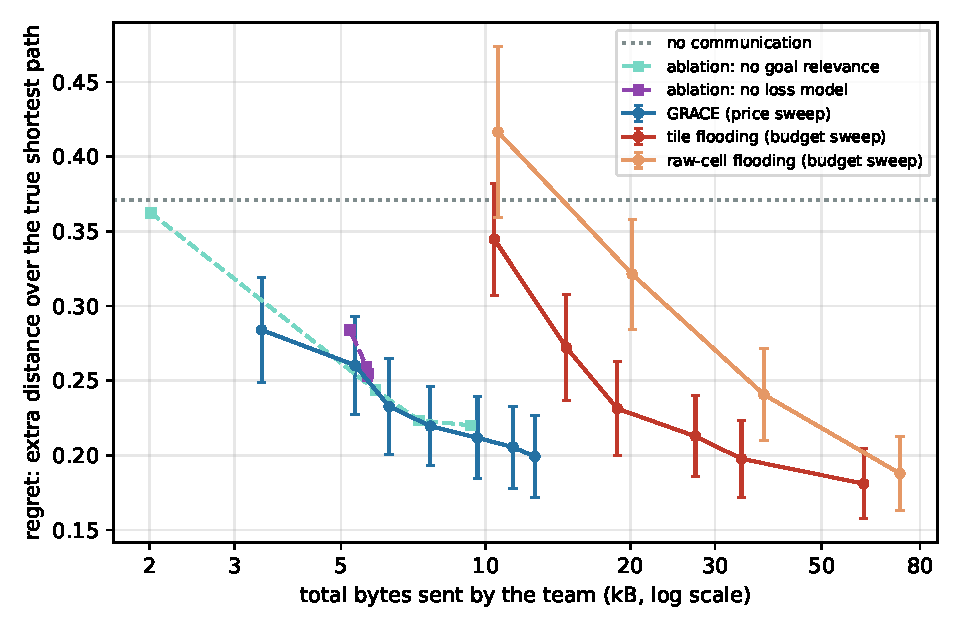
\includegraphics[width=0.72\linewidth]{fig/pareto.pdf}
\caption{Bytes against detour. Each curve sweeps its knob: price for GRACE, per-slot budget for flooding.}
\label{fig:pareto}
\end{figure}

\paragraph{Bytes for the same detour (Figure~\ref{fig:pareto}).} Silence costs a mean regret of $0.371$. GRACE matches the regret of tile flooding with \textbf{2.9--3.3$\times$ fewer bytes}: paired over seeds, GRACE at $\kappa=0.2$ against flooding at 24 B/slot differs by $-0.001\pm0.013$ in regret, with $3.1\times$ fewer bytes (9.6 against 27.3 kB). Against raw-cell flooding the saving is about $6\times$, as Corollary~\ref{cor:tile} predicts for the code alone combined with the scheduling. The information efficiency $\eta$ (regret removed per kB) is $0.013$--$0.026$ for GRACE against $0.002$--$0.007$ for tile flooding. The lowest regret is reached by flooding at 64 B/slot ($0.181$, 61 kB); GRACE's best is $0.199$ with $5.1\times$ fewer bytes, a paired difference of $0.018\pm0.010$. Raw-cell flooding with a small budget ($0.417$) is no better than silence: partial, unprioritised obstacle knowledge can push optimistic planners into unexplored pockets.

\paragraph{What each component buys.} Without the loss model, the protocol sends each tile once and never repairs a loss: its curve stalls at a regret of $0.253$ whatever the price, while GRACE keeps converting bytes into lower regret down to $0.199$. Without goal relevance, the curve lies on GRACE's own front within error bars in this scenario. We therefore cannot claim a measurable benefit of goal relevance \emph{for transmission} here: with a short convoy along similar routes, most tiles are relevant to someone. Relevance does matter for memory (next paragraph).

\begin{figure}[t]\centering
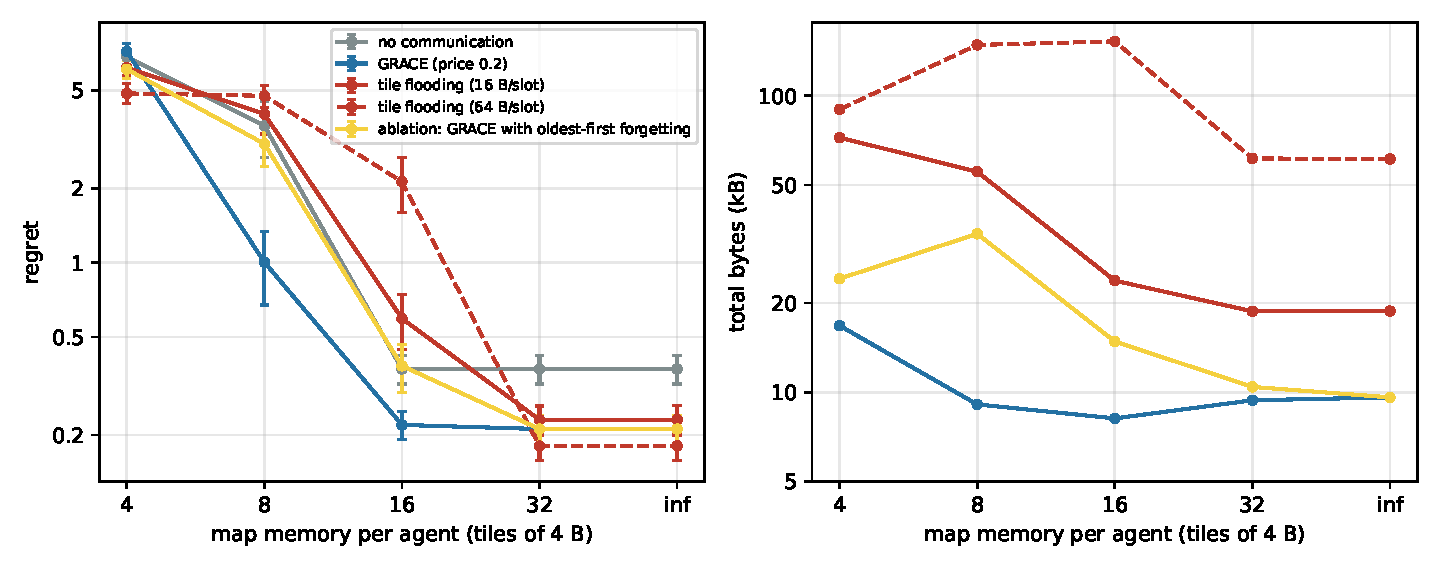
\includegraphics[width=\linewidth]{fig/memory.pdf}
\caption{Bounded map memory. Left: regret (log scale). Right: bytes. One tile is 4 bytes.}
\label{fig:memory}
\end{figure}

\paragraph{Bounded memory (Figure~\ref{fig:memory}).} With 16 tiles (64 bytes of map memory) per agent, GRACE stays at its unlimited-memory regret ($0.220$ against $0.212$) with full arrival. With the same memory, tile flooding degrades from $0.231$ to $0.594$ (16 B/slot) and from $0.181$ to $2.13$ (64 B/slot), worse than silence, with 18\,\% of agents not arriving: incoming tiles that do not matter evict the ones that do, and agents loop. Replacing ellipse-margin forgetting by oldest-first forgetting in GRACE raises the regret to $0.382$, so the relevance-aware memory rule of Corollary~\ref{cor:forget} accounts for most of the difference. At 8 tiles, GRACE keeps 89\,\% of agents arriving, against 60\,\% for silence and 43--59\,\% for flooding. At 4 tiles every protocol fails, because an agent cannot even hold the pocket it is standing in.

\begin{figure}[t]\centering
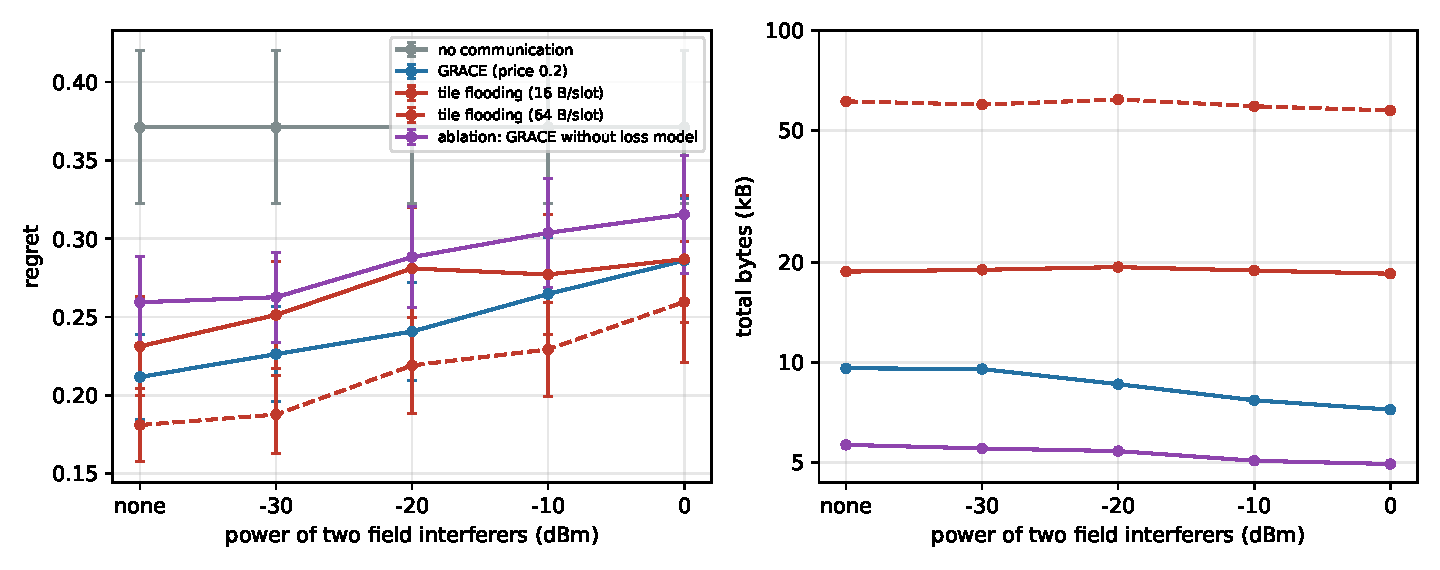
\includegraphics[width=\linewidth]{fig/interference.pdf}
\caption{Two field interferers near the middle of every route, increasing power.}
\label{fig:interference}
\end{figure}

\paragraph{Interference (Figure~\ref{fig:interference}).} As the interferers grow from off to 0 dBm, every protocol loses part of its benefit. GRACE's regret rises from $0.212$ to $0.286$, which equals tile flooding at 16 B/slot ($0.287$) with $2.6\times$ fewer bytes. Without being told anything, GRACE \emph{spends less} as the channel degrades (9.6 to 7.2 kB): fewer teammates are heard and \eqref{eq:beta} makes copies into bad links look less valuable. Flooding keeps spending the same. The ablation without the loss model is worse at every interference level.

\begin{figure}[t]\centering
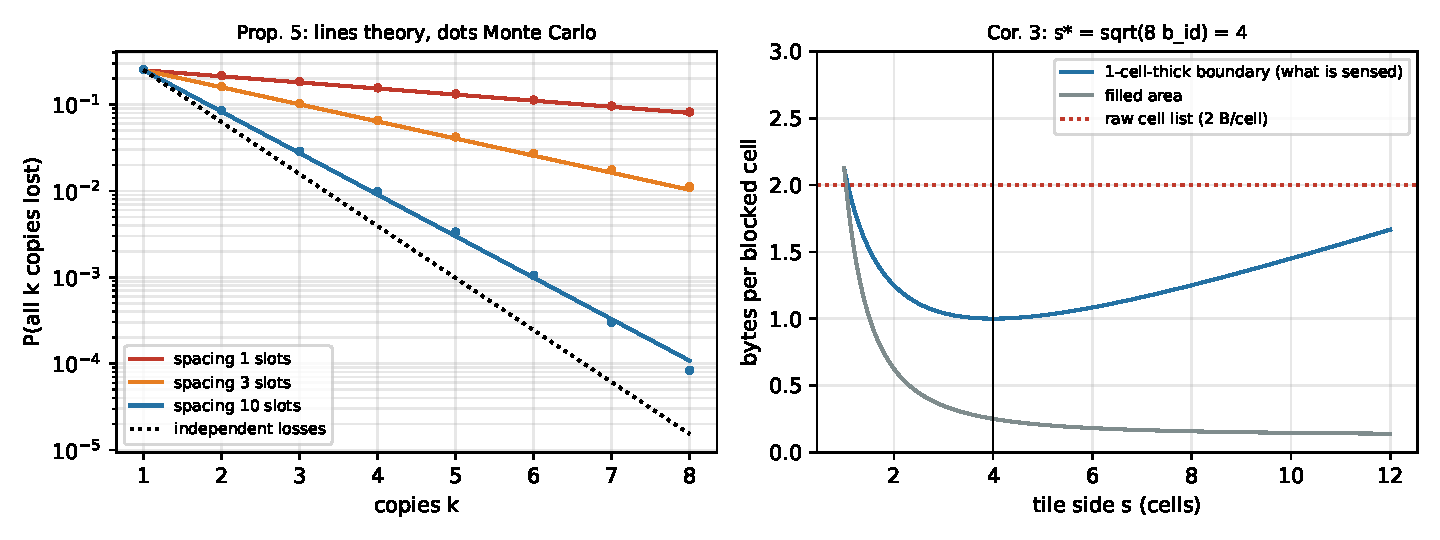
\includegraphics[width=\linewidth]{fig/theory_checks.pdf}
\caption{Left: Proposition~\ref{prop:allLost} (lines) against Monte Carlo simulation of the chain (dots), $\pi_B=0.25$, mean outage 6.7 slots. Right: bytes per blocked cell against tile side (Corollary~\ref{cor:tile}).}
\label{fig:theory}
\end{figure}

\paragraph{Theory checks (Figure~\ref{fig:theory}).} The closed form of Proposition~\ref{prop:allLost} matches Monte Carlo over four orders of magnitude, and shows that one-slot repetition on a bursty link barely helps. The test suite also checks Proposition~\ref{prop:cond}, $k^\star$ (Proposition~\ref{prop:kstar}) against brute force, Lemma~\ref{lem:tiles} exactly, Lemma~\ref{lem:ellipse} and Proposition~\ref{prop:voi} on random terrains, the memory bound, and that the agent code cannot import the world.
